\section{Modeling Metabolites using EKF}
\label{Modeling Metabolites using EKF}

\noindent This example is inspired by research that models the biological pathway of metabolites, which are molecules that are the byproduct of the body's metabolism. This model contains four different states, or metabolites, which contain 18 unknown parameters \cite{article5}. Unlike the original research, which had datasources of their own, this example will simulate data by using a built-in ODE solver on Matlab. Ultimately, the two goals of this example is to demonstrate how the EKF can be applied, how the EKF can correct for multiple variables or states, and how the EKF can be used for parameter fitting. \\ 

\noindent In this example, the four metabolites, or states, have the following differential equations:
\begin{align*}
\dot x_1 &= \alpha_1 x_3^{g_{13}} x_5^{g_{15}} - \beta_1 x_1^{h_{11}}, \\
\dot x_2 &= \alpha_2 x_1^{g_{21}} - \beta_2 x_2^{h_{22}}, \\
\dot x_3 &= \alpha_3 x_2^{g_{32}} - \beta_3 x_3^{h_{33}} x_4^{h_{34}}, \\
\dot x_4 &= \alpha_4  x_1^{g_{41}} - \beta_4 x_4^{h_{44}},
\end{align*}
where there are 18 unknown parameters ($\alpha_1, \hdots, \alpha_4, \beta_1, \hdots, \beta_4, g_{13}, g_{15}, g_{21}, \\ g_{32}, g_{41}, h_{11}, h_{22}, h_{33}, h_{34}, h_{44} $). Therefore, the state vector is given by $x_k = [x_{1,k}, x_{2,k}, x_{3,k}, x_{4,k}]^T$. We will use the EKF to find parameter values that best fit this model to its true states. In both the original example as well as this one, sampling time will be 0.1 seconds for 5 seconds, totaling 50 UKF estimates. Since we did not have access to the original example's dataset, data is simulated on MATLAB. Similar to the previous example, the system's true output was simulated using an ODE solver and incoming system measurements were calculated by adding noise to the true value. The model was initialized by setting the state variable to $x_0 = [4, 1, 3, 4]^T$ and the state covariance to $P_0 = .01I$. 

\subsubsection{Implementing EKF}

\noindent These states are given in a continuous state space model and need to be discretized. Recall that a continuous state space given by $\dot x(t) = Ax(t)$ can be discretized into $x_k = e^{At}x_{k-1}$. Here, our transition matrix, $A$, is not unique. One value for $A$, includes:
%\begin{align*}
%\dot x(t) = Ax(t)
%\end{align*}
$$
\scriptsize{
\begin{bmatrix}
-b1*x_1^{h_{11}-1} & 0 & x_5*x(3)^{g_{13}-1}& 0 & 0  & 0 & 0  & 0 \\
x_6*x(1)^{g_{21}-1} & -b2*x_2^{h_{22}-1}&0&0&0&0&0&0 \\
0&x_7*x_2^{g_{32}-1}&-b3*x_3^{h_{33}-1}*x_4^{h_{34}}&0&0&0&0&0\\
0&0&0&-b4*x_4^{h_{44}-1}&0&0&0&x_1^{g_{41}}\\
\end{bmatrix}}.
$$


\begin{figure}[h]
    \centering
    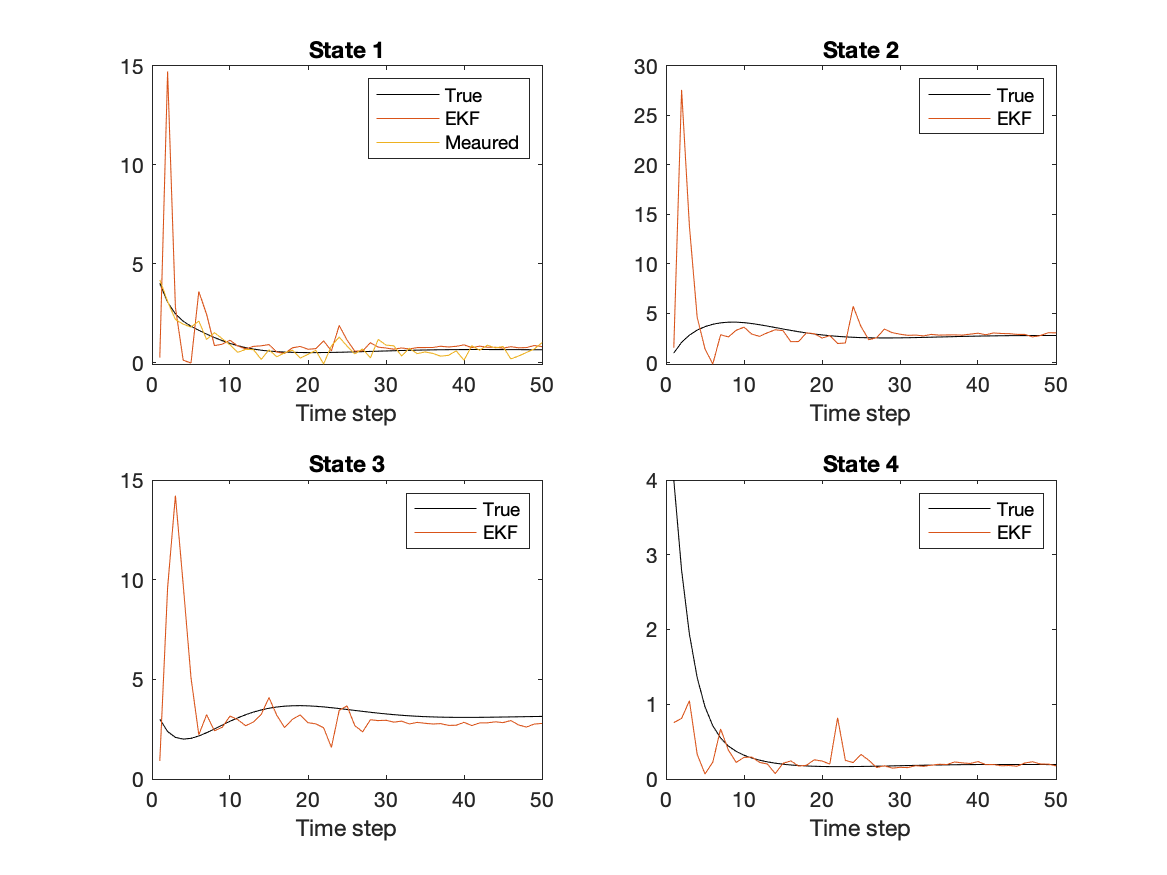
\includegraphics[scale = 0.6]{EKF_1_state.png}
    \caption{sdaasads}
\end{figure}

\subsubsection{EKF multiple state correction}

\subsubsection{EKF Parameter Estimation}

$$
\scriptsize{
\begin{bmatrix}
-b1*x_1^{h_{11}-1} & 0 & x_5*x(3)^{g_{13}-1}& 0 & 0  & 0 & 0  & 0 \\
x_6*x(1)^{g_{21}-1} & -b2*x_2^{h_{22}-1}&0&0&0&0&0&0 \\
0&x_7*x_2^{g_{32}-1}&-b3*x_3^{h_{33}-1}*x_4^{h_{34}}&0&0&0&0&0\\
0&0&0&-b4*x_4^{h_{44}-1}&0&0&0&x_1^{g_{41}}\\
0&0&0&0&0&0&0&0 \\
0&0&0&0&0&0&0&0 \\
0&0&0&0&0&0&0&0 \\
0&0&0&0&0&0&0&0 \\
\end{bmatrix}}.
$$
\begin{center}
\begin{table}

\caption{True Parameter Values} \label{tab:sometab}
\begin{tabular}{ |P{1cm}||P{1cm} P{1cm} P{1cm} P{1cm} P{1cm} P{1cm} P{1cm} P{1cm} P{1cm} P{1cm}|}
    \hline
    \multicolumn{11}{|c|}{True Parameter Values} \\ 
    \hline
      & $\alpha_i$ & $g_{i1}$ & $g_{i2}$ & $g_{i3}$ & $g_{i4}$ & $\beta_i$ & $h_{i1}$ & $h_{i2}$ & $h_{i3}$ & $h_{i4}$\\
    \hline
    $x_1$ & 20.0  & 0 & 0 & -0.8 & 0 & 10.0 & 0.5 & 0 & 0 & 0\\
    $x_2$ & 8.0  & .5  & 0 & 0 & 0 & 3.0 & 0 & 0.75 & 0 & 0\\
    $x_3$ & 3.0  & 0 & 0.75 & 0 & 0 & 5.0 & 0 & 0 & 0.5 & 0.2\\
    $x_4$ & 2.0 & .5  & 0 & 0 & 0 & 6.0 & 0 & 0 & 0 & 0.8\\
    
    \hline
\end{tabular}
\end{table}
\end{center}


\begin{figure}[h]
    \centering
    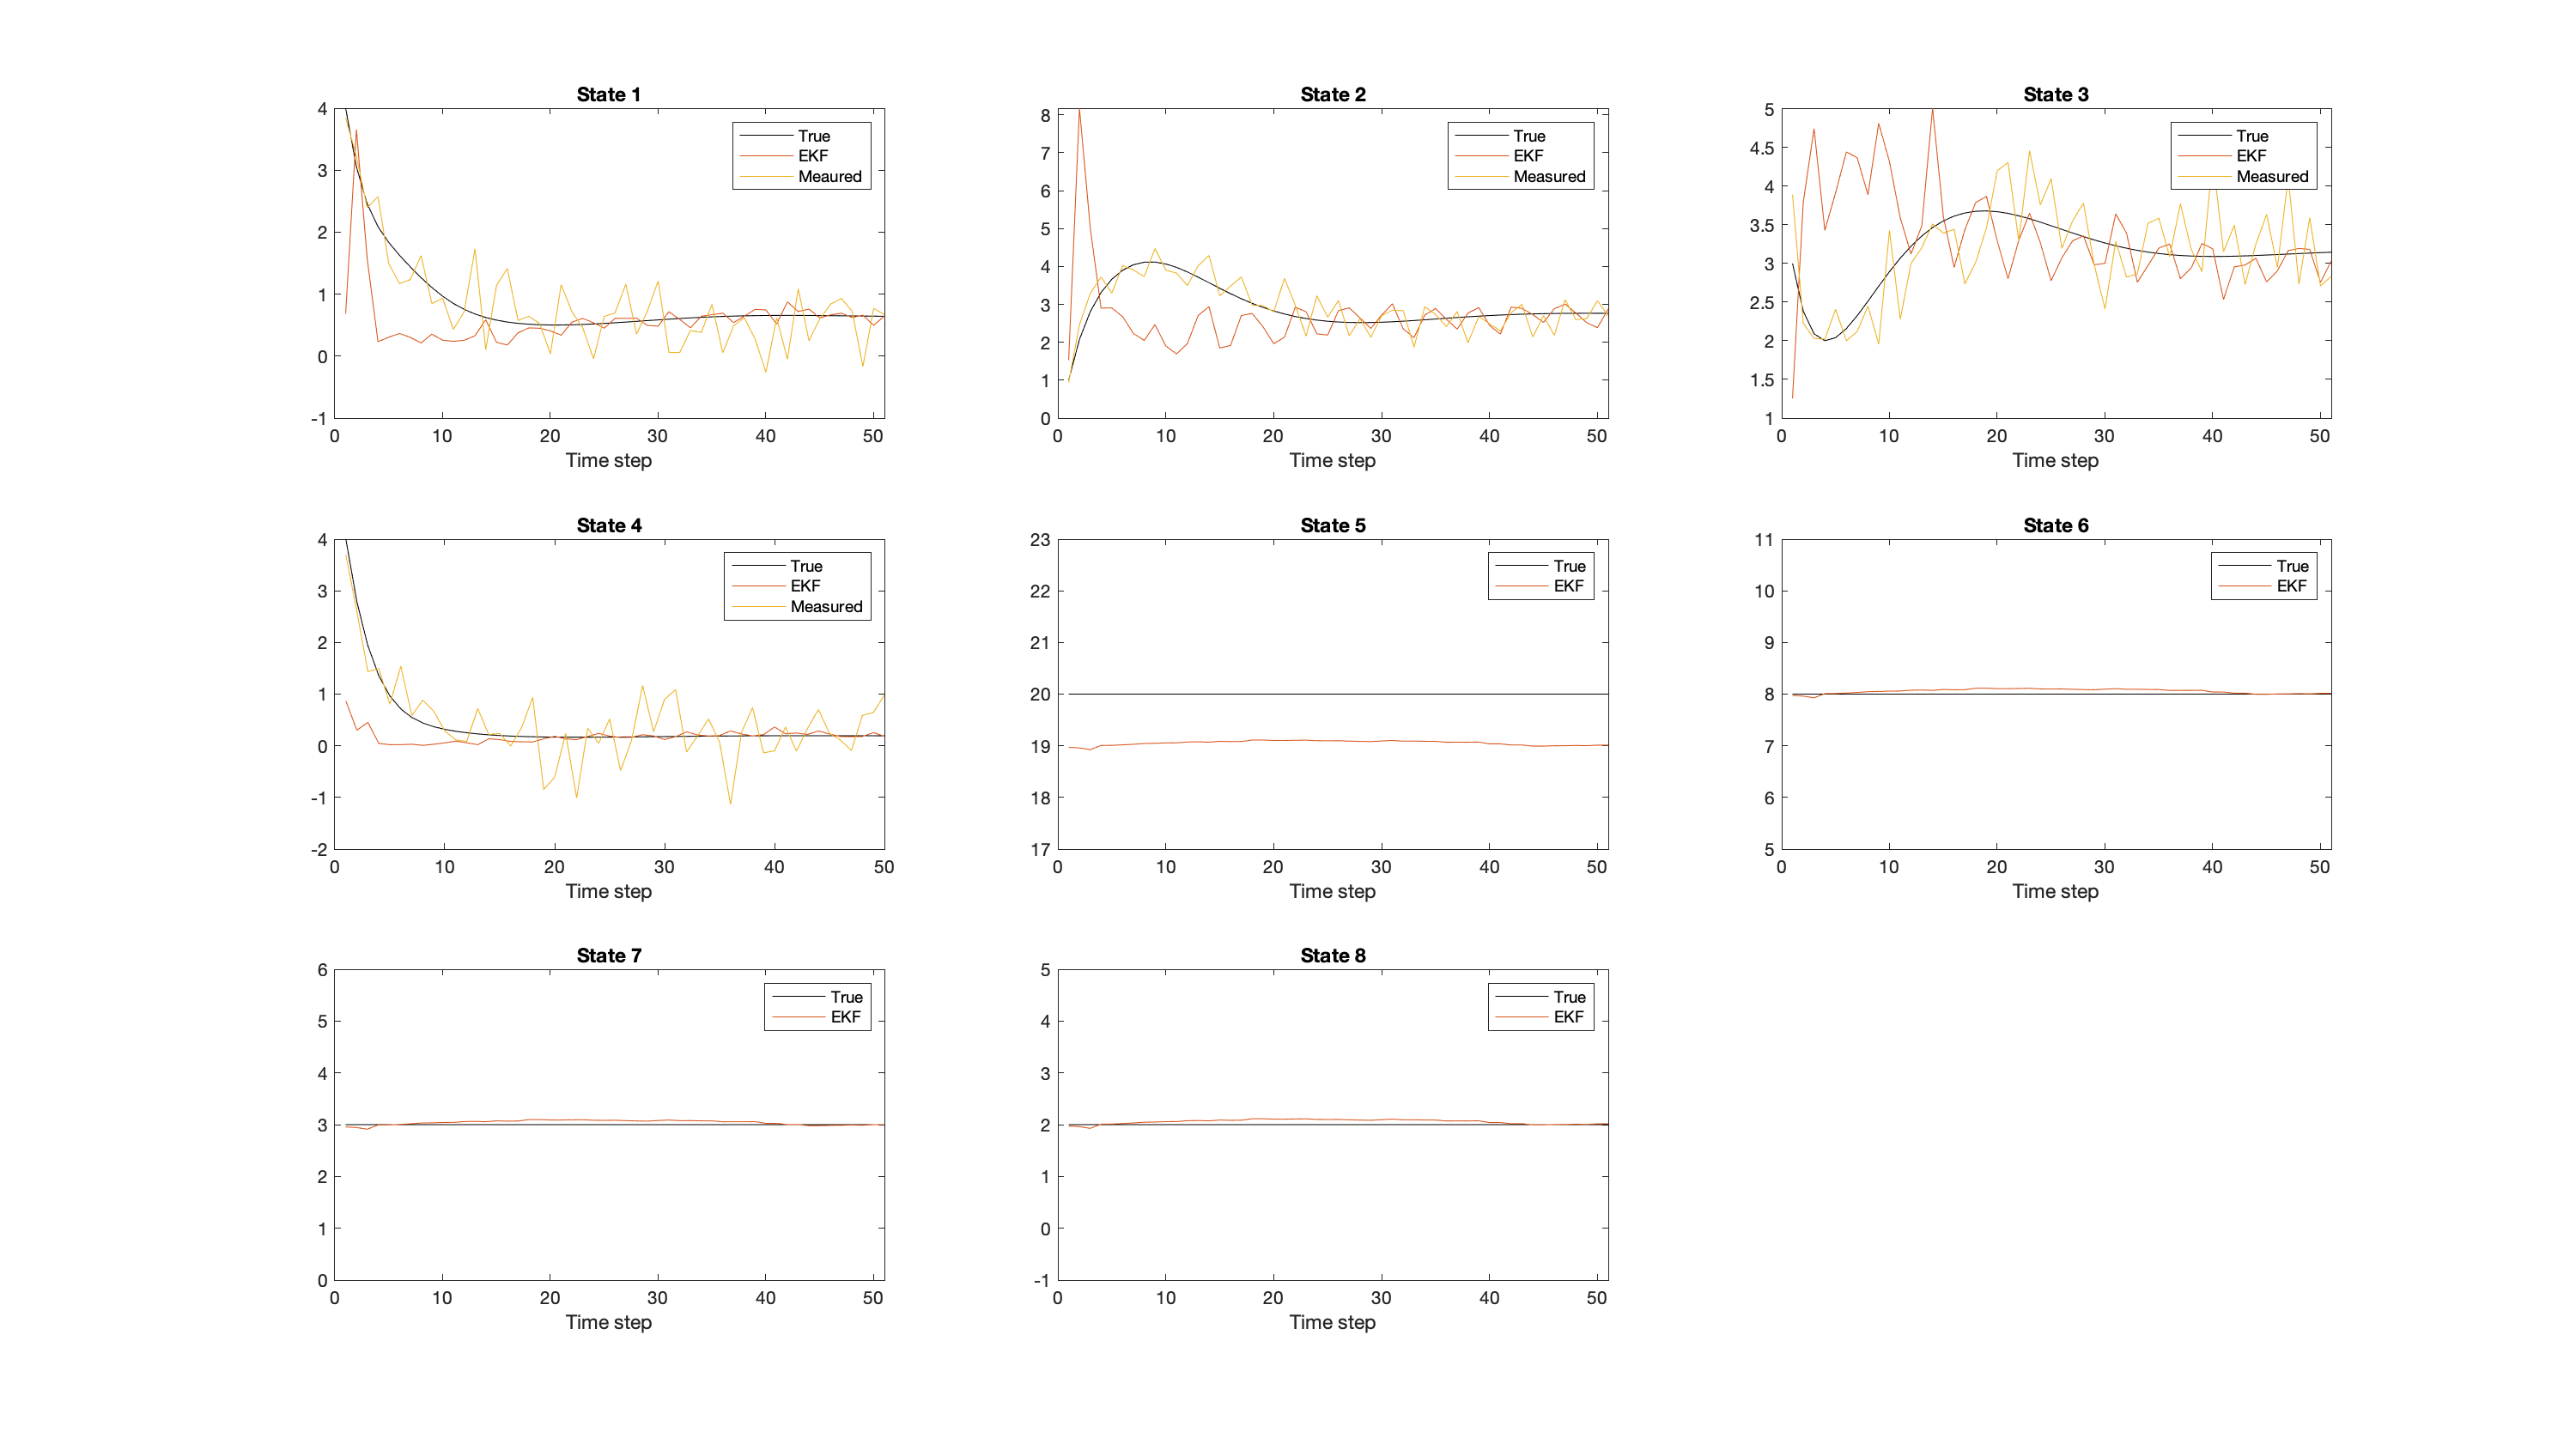
\includegraphics[scale = 0.6]{EKF_param_est.png}
    \caption{sdaasads}
\end{figure}


\noindent Residuals, also known as the innovation, are one way to access the model's performance. Recall that the residual is the difference between the actual measurement values and the predicted measurement values. Since only one state, $x1$ had incoming measurements, the residual graph in Figure 4.10 is specifically for $x1$. Generally, a strong residual graph has

\begin{itemize}
\item a symmetrical distribution that is clustered toward the center,
\item values that are close to 0,
\item a random or unclear pattern.
\end{itemize}


\textcolor{red}{ADD RESIDUAL GRAPH HERE}
\begin{figure}[h]
    \centering
    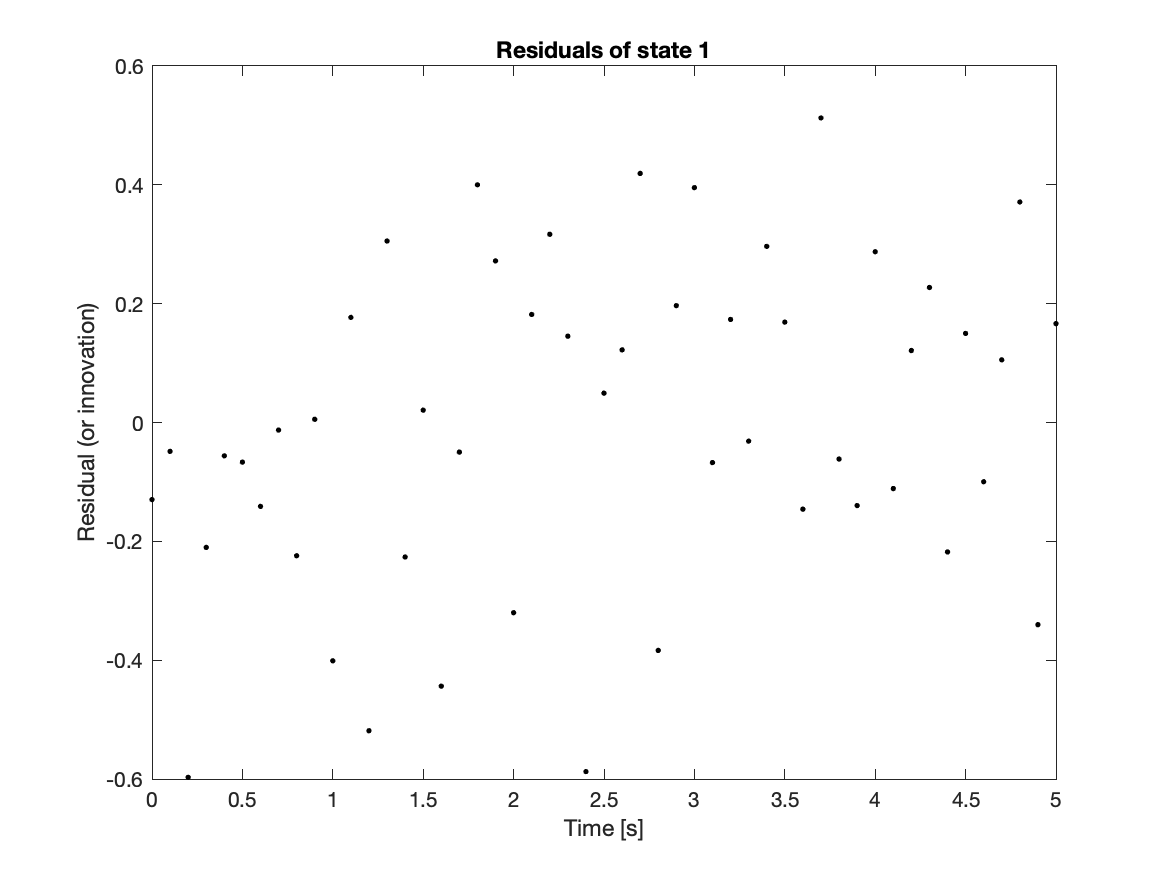
\includegraphics[scale = 0.6]{Meskin_residuals_state1.png}
    \caption{This scatterplot provides information regarding the residual, or innovation, of the first state, which is the only state recieving incoming system measurements.}
\end{figure}














